\chapter{Laboratorio 4}
\section{Introduzione}
Durante questa attività di laboratorio si è dapprima terminata l'analisi del circuito common emitter amplifier e in seguito si è introdotto l'utilizzo del amplificatore operazionale \textmu A741 (datasheet \url{https://www.ti.com/lit/ds/symlink/ua741.pdf}), utilizzato nella configurazione di amplificatore invertente e integratore.

\section{Common emitter amplifier: analisi capacità di disaccoppiamento in ingresso}
Si consideri l'analisi di piccolo segnale del circuito common emitter amplifier con alimentazione singola già presentata (capitolo \ref{sec:33}), considerando però ora anche la capacità di disaccoppiamento C (\Fig\ref{fig:commonemitter_se_c_AC}).
\begin{figure}[h!]
	\centering
	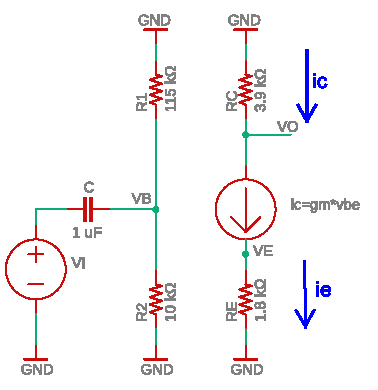
\includegraphics[width=0.4\linewidth]{./OtherFiles/Laboratorio 4/common emitter_se_c-piccolo segnale-printout}
	\caption{Analisi per piccolo segnale del circuito common emitter amplifier con alimentazione singola.}
	\label{fig:commonemitter_se_c_AC}
\end{figure}

Le resistenze R\sub{1} e R\sub{2} sono in parallelo, poiché connesse tra il nodo v\sub{b} e massa. Esse possono quindi essere sostituite con una resistenza e equivalente di valore $R_{12}=R_1 // R_2=\frac{R_1*R_2}{R_1+R_2}$.

Svolgendo un bilancio di correnti al nodo V\sub{b}, siamo in grado di definire l'andamento della tensione nel nodo v\sub{b} nel dominio delle trasformate di Laplace:
\begin{equation}
	\begin{split}
		i_C(s)&=i_R(s) \\
		\frac{v_i(s)-v_b(s)}{Z_C(s)}&=\frac{v_b(s)-\SI{0}{\volt}}{R_{12}} \\
		\frac{v_i(s)-v_b(s)}{\frac{1}{sC}}&=\frac{v_b}{R_{12}} \\
		(v_i(s)-v_b(s))sC&=\frac{v_b}{R_{12}} \\
		\text{da cui si ricava} \\
		v_b(jw)&=\frac{jwR_{12}C}{1+jwR_{12}C}v_i.
	\end{split}
\end{equation}
L'equazione ricavata corrisponde all'equazione di un filtro passa-alto. Per cui, se $w>>w_C=\frac{1}{R_{12}C}$ allora v\sub{b}=v\sub{i}, ossia il condensatore può essere considerato un corto. Calcolando la pulsazione critica w\sub{C} con i valori delle resistenze del nostro circuito otteniamo $w_C\simeq \SI{107.5}{\radian/\second}$ che equivale a una frequenza di $f_C\simeq\SI{17.1}{\hertz}$.

Di seguito è riportato il diagramma di Bode reale del modulo della funzione di trasferimento che lega v\sub{i} e v\sub{b} (\Fig\ref{fig:hpf}). Dal grafico si può ricavare che la w\sub{C} è di \SI{109}{\radian/\second}, simile a quella calcolata in modo approssimativo. 
\begin{figure}[h!]
	\centering
	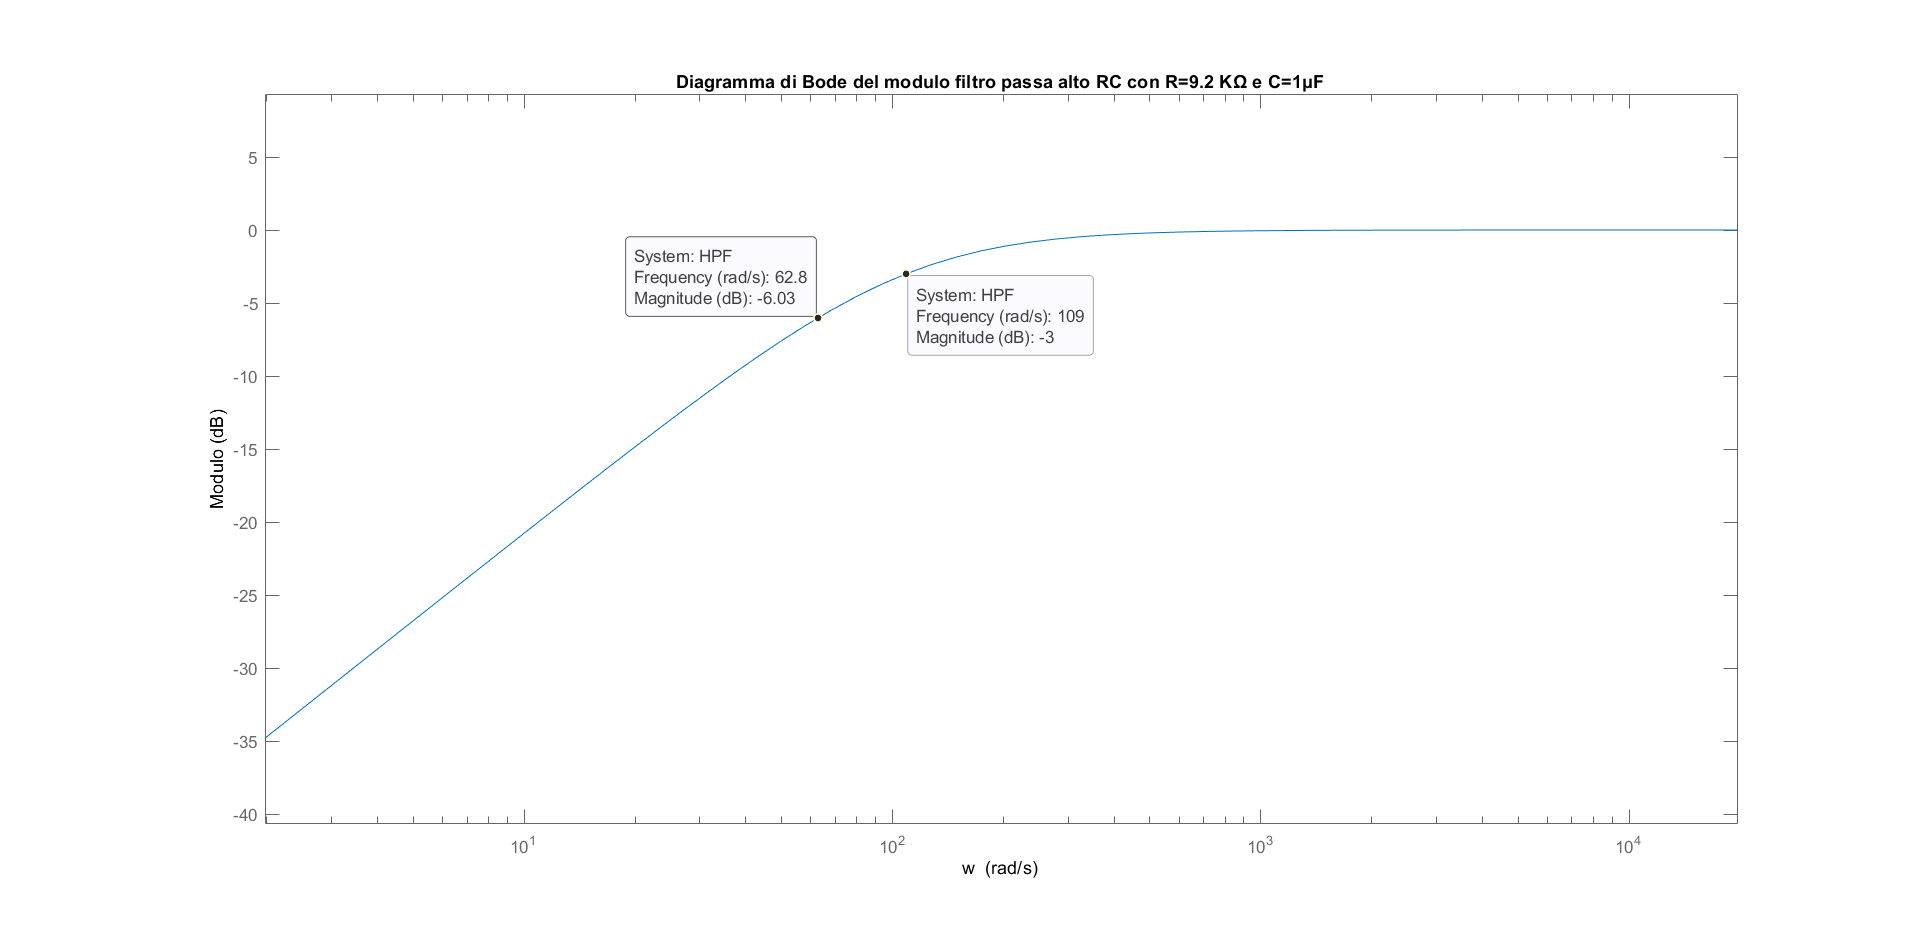
\includegraphics[width=1\linewidth]{./OtherFiles/Laboratorio 4/boderc.png}
	\caption{Diagramma di Bode del modulo del filtro RC passa-alto, con R=\SI{9.2}{\kilo\ohm} e C=\SI{1}{\micro\farad}.}
	\label{fig:hpf}
\end{figure}

In laboratorio è stato possibile misurare la tensione al nodo v\sub{i} in ingresso e la tensione sul nodo v\sub{b}, con un segnale sinusoidale di frequenza \SI{10}{\hertz} e ampiezza picco-picco di \SI{100}{\milli\volt}. Nella figura \ref{fig:hpf_10hz} sono riportati i risultati. Come ci aspettavamo, essendo al di sotto della pulsazione critica ($w\simeq\SI{62.8}{\radian/\second}$) il segnale risulta essere attenuato di circa \SI{4.2}{\decibel}. Si noti che il segnale risulta essere molto rumoroso, in quanto l'oscilloscopio presenta difficoltà nel misurare segnali con frequenza così bassa. Per questo, anche le misure ricavate dall'esperimento risultano essere soggette a rumore. Tuttavia, questo risultato è compatibile con il digramma di Bode del modulo sopra descritto, il quale indica un valore di attenuazione pari a \SI{-6}{\decibel}. Inoltre, si può notare anche l'introduzione di uno sfasamento tra i segnali in ingresso e in uscita, introdotto dal filtro passa alto e verificabile con il digramma della fase.
\begin{figure}[h!]
	\centering
	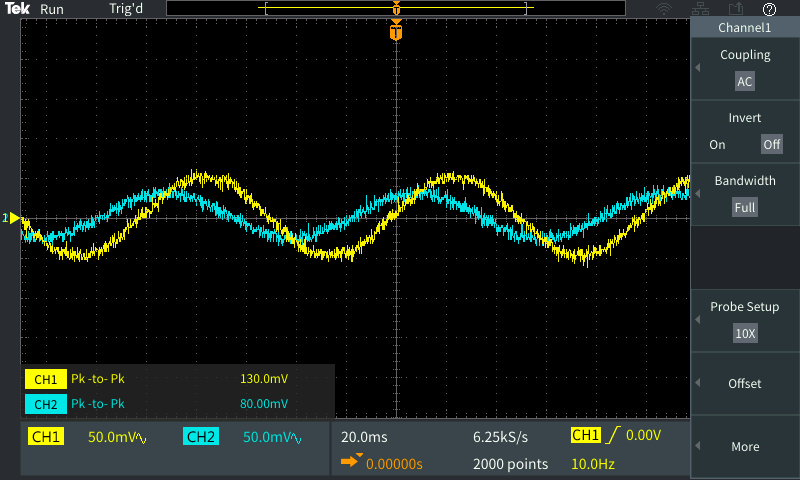
\includegraphics[width=0.6\linewidth]{./ImageFiles/Laboratorio 4/TEK00003}
	\caption{Confronto tra il segnale in ingresso (CH1) al condensatore e in uscita (CH2) sul nodo v\sub{i} con segnale sinusoidale di ampiezza picco-picco \SI{100}{\milli\volt} e frequenza \SI{10}{\hertz}.}
	\label{fig:hpf_10hz}
\end{figure}

\section{Amplificatore operazionale \textmu A741}
La successiva esperienza consisteva nel realizzare un amplificatore invertente utilizzando l'amplificatore operazionale \textmu A741, realizzando il seguente circuito:
\begin{figure}[h!]
	\centering
	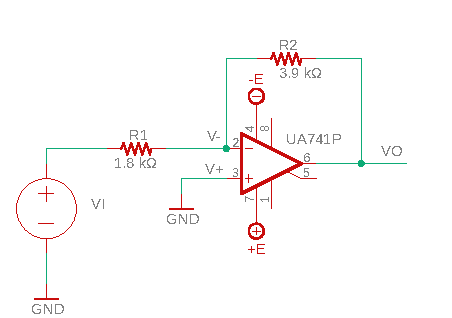
\includegraphics[width=0.6\linewidth]{./OtherFiles/Laboratorio 4/opam_inv}
	\caption{Amplificatore operazionale in configurazione invertente.}
	\label{fig:opamp_inv}
\end{figure}
In particolare, per le resistenze R\sub{1} e R\sub{2} sono state utilizzate le resistenze utilizzate nel circuito precedente. Le tensioni di alimentazione +E e -E sono state inizialmente impostate a \SI{+10}{\volt} e \SI{-10}{\volt}.

\begin{figure}[h!]
	\centering
	\includegraphics[width=0.6\linewidth]{./ImageFiles/Laboratorio 4/IMG\_20220531\_113527\_2}
	\caption{Circuito realizzato con amplificatore operazionale in configurazione invertente.}
	\label{fig:opamp_inv_circuito}
\end{figure}

Analizzando il circuito, è facilmente ricavabile che 
\begin{equation}
	V_O=-\frac{R_2}{R_1}V_i
\end{equation}
tramite un bilancio di corrente nel nodo V\textsuperscript{+} e ricordando che, in presenza di una reazione negativa, V\textsuperscript{+}=V\textsuperscript{-}. Con i valori di resistenze utilizzate, ci aspettiamo un guadagno di circa 2.17.